\documentclass[aspectratio=169, table]{beamer}

\usepackage{colortbl}
\usepackage{xcolor}
\usepackage{listings}
\usepackage{tikz}
\usepackage{pgfplots}
\usepgfplotslibrary{polar}
\usetikzlibrary{arrows.meta, positioning, calc}

\usetheme{Pradita}


\usepackage{listings}
\lstdefinestyle{SqlStyle}{
language=SQL,
basicstyle=\ttfamily\footnotesize,
morekeywords={REAL, TEXT, REFERENCES},
keywordstyle=\color{blue},
commentstyle=\color{gray},
stringstyle=\color{red},
breaklines=true,
showstringspaces=false,
tabsize=2,
captionpos=b,
numbers=left,
numberstyle=\tiny\color{gray},
frame=lines,
backgroundcolor=\color{lightgray!10},
comment=[l]{//},
morecomment=[s]{/*}{*/},
commentstyle=\color{gray}\ttfamily,
string=[s]{'}{'},
morestring=[s]{"}{"},
%	stringstyle=\color{teal}\ttfamily,
%	showstringspaces=false
}

\lstdefinelanguage{bash} {
keywords={},
basicstyle=\ttfamily\small,
keywordstyle=\color{blue}\bfseries,
ndkeywords={iex},
ndkeywordstyle=\color{purple}\bfseries,
sensitive=true,
commentstyle=\color{gray},
stringstyle=\color{red},
numbers=left,
numberstyle=\tiny\color{gray},
breaklines=true,
frame=lines,
backgroundcolor=\color{lightgray!10},
tabsize=2,
comment=[l]{\#},
morecomment=[s]{/*}{*/},
commentstyle=\color{gray}\ttfamily,
stringstyle=\color{purple}\ttfamily,
showstringspaces=false
}

% Define Java language style for listings
\lstdefinestyle{JavaScript}{
	language=Java,
	basicstyle=\ttfamily\footnotesize,
	keywordstyle=\color{blue},
	commentstyle=\color{gray},
	stringstyle=\color{red},
	breaklines=true,
	showstringspaces=false,
	tabsize=4,
	captionpos=b,
	numbers=left,
	numberstyle=\tiny\color{gray},
	frame=lines,
	backgroundcolor=\color{lightgray!10},
	comment=[l]{//},
	morecomment=[s]{/*}{*/},
	commentstyle=\color{gray}\ttfamily,
	string=[s]{'}{'},
	morestring=[s]{"}{"},
	%	stringstyle=\color{teal}\ttfamily,
	%	showstringspaces=false
}

\title{\Huge Text \& Sentiment \\
\vspace{10pt}
 Analysis}
\subtitle{IT140704 - Big Data for Business}
%\date[Serial]{Penggunaan Large Language Model untuk Pengajaran}
\author{\textbf{Alfa Yohannis}}
\begin{document}

\frame{\titlepage}


\begin{frame}[fragile]
\frametitle{Contents}
\vspace{20pt}
\begin{columns}[t]
	\column{0.5\textwidth}
	\tableofcontents[sections={1-5}]
	
	\column{0.5\textwidth}
	\tableofcontents[sections={6-20}]
\end{columns}
\end{frame}

\begin{frame}{\hfill}
	\centering
	\Huge{\textbf{How can text generated by clients be used to create real strategic, tactical, and operational values?}}
\end{frame}


\section{Introduction to Text \& Sentiment Analysis}

\begin{frame}{Introduction to Text \& Sentiment Analysis}
	\vspace{20pt}
	\begin{itemize}
		\item \textbf{Text Analysis:} NLP branch for processing, extracting information, and finding patterns in text data.
		\item \textbf{Data Sources:} reviews, social media, emails, forums, news, internal documents.
		\item \textbf{Sentiment Analysis:} identifies and classifies opinions/emotions as positive, negative, neutral, or scored (-1 to +1).
		\item \textbf{Business Applications:} brand monitoring, crisis prevention, marketing evaluation, trend detection.
		\item \textbf{Methods:} lexicon-based, machine learning (e.g., Logistic Regression, SVM), deep learning (LSTM, BERT).
		\item \textbf{Challenges:} language ambiguity, sarcasm, code-switching, domain dependency.
	\end{itemize}
\end{frame}

\section{Business Applications \& Sentiment Analysis}
\begin{frame}{Business Applications \& Sentiment Analysis}
	\vspace{20pt}
	\begin{itemize}
		\item \textbf{E-commerce:} Identify product strengths/weaknesses from customer reviews; inform product improvement and post-sales service.
		\item \textbf{Banking \& Finance:} Monitor market sentiment; detect shifts in investor confidence for faster portfolio adjustments.
		\item \textbf{Tourism \& Hospitality:} Track guest feedback to enhance service quality and build a strong reputation.
		\item \textbf{Retail:} Detect emerging product trends via social media before they appear in sales data.
		\item \textbf{Government:} Measure public reaction to policies; adapt communication for better acceptance.
		\item \textbf{Predictive Insights:} Anticipate consumer behavior changes and enable proactive strategy.
	\end{itemize}
\end{frame}

\section{Popular Methods}

\begin{frame}{Popular Techniques and Methods}
	\vspace{20pt}
	\begin{enumerate}
		\item \textbf{Lexicon-based Approach:} Uses predefined dictionaries with sentiment scores; simple, no large labeled dataset needed; limited by context understanding.
		\item \textbf{Machine Learning-based Approach:} Trains classifiers (e.g., Naive Bayes, Logistic Regression, SVM) on labeled data; adaptable to domain-specific language.
		\item \textbf{Deep Learning-based Approach:} Leverages neural networks (LSTM, CNN, Transformers) to capture semantic and syntactic context; high accuracy but resource-intensive.
		\item \textbf{Method Selection:} Depends on labeled data availability, desired accuracy, and computational resources; hybrid systems often combine strengths.
	\end{enumerate}
\end{frame}


\begin{frame}{Methods: Lexicon-based Approach}
	\vspace{20pt}
	\begin{itemize}
		\item Uses predefined dictionaries of words/phrases with sentiment scores or labels.
		\item Matches text tokens to lexicon entries and aggregates scores.
		\item \textbf{Advantages:} Simple, no need for large labeled datasets, quick to implement.
		\item \textbf{Limitations:} Struggles with ambiguity, sarcasm, and complex context.
		\item Popular resources: SentiWordNet, AFINN, VADER (optimized for informal/social media text).
		\item Suitable for rapid sentiment estimation in low-resource scenarios.
	\end{itemize}
\end{frame}

\begin{frame}{Methods: Machine Learning-based Approach}
	\vspace{20pt}
	\begin{itemize}
		\item Uses labeled datasets and classification algorithms to learn sentiment patterns.
		\item Workflow: data collection $\rightarrow$ preprocessing (tokenization, normalization) → feature extraction (BoW, TF–IDF) $\rightarrow$ model training $\rightarrow$ evaluation.
		\item Common algorithms: Naive Bayes, Logistic Regression, SVM, Random Forest.
		\item \textbf{Advantages:} Adapts to domain-specific language; high accuracy with sufficient data.
		\item \textbf{Limitations:} Needs large, representative datasets; performance drops on unseen domains without retraining.
	\end{itemize}
\end{frame}

\begin{frame}{Methods: Deep Learning-based Approach}
	\vspace{20pt}
	\begin{itemize}
		\item Uses neural network architectures to capture semantic and syntactic relationships in text.
		\item Common architectures: LSTM, GRU (sequential data), CNN (local features), Transformers (BERT, RoBERTa, XLNet).
		\item \textbf{Advantages:} High accuracy; handles complex, contextual language well; can fine-tune pre-trained models with less data.
		\item \textbf{Limitations:} Requires significant computational resources and longer training times.
		\item Often used in hybrid systems to combine strengths of multiple approaches.
	\end{itemize}
\end{frame}


\section{Text \& Sentiment Analysis Workflow}

\begin{frame}{Text \& Sentiment Analysis Workflow}
	\vspace{20pt}
	\begin{enumerate}
		\item \textbf{Data Collection:} Gathering text from internal (emails, feedback) and external sources (social media, reviews, public datasets).
		\item \textbf{Text Preprocessing:} Cleaning and normalizing text (tokenization, stopword removal, stemming/lemmatization, handling emojis/hashtags).
		\item \textbf{Feature Extraction:} Converting text to numerical form (Bag-of-Words, TF-IDF (Term Frequency – Inverse Document Frequency), embeddings like Word2Vec, BERT (Bidirectional Encoder Representations from Transformers)).
		\item \textbf{Sentiment Classification:} Assigning categories (positive, negative, neutral) using ML/DL algorithms.
		\item \textbf{Model Evaluation:} Measuring performance with accuracy, precision, recall, F1-score, confusion matrix, ROC/AUC.
	\end{enumerate}
\end{frame}

\begin{frame}{Data Collection \& Sentiment Analysis}
	\vspace{20pt}
	\begin{itemize}
		\item Sources: internal (emails, feedback forms, call transcripts) and external (e-commerce reviews, social media, forums, news, public datasets).
		\item Methods: manual collection, structured data import (CSV/DB), \textit{web scraping} (BeautifulSoup, Scrapy), APIs (Twitter, Reddit, Google Reviews).
		\item Public datasets: e.g., \textit{Sentiment Labelled Sentences} from UCI ML Repository.
		\item Quality factors: avoid bias, ensure representativeness, maintain class balance for reliable model performance.
	\end{itemize}
\end{frame}

\begin{frame}{Text Preprocessing}
	\vspace{20pt}
	\begin{itemize}
		\item Purpose: clean and prepare raw text for analysis, removing irrelevant elements (punctuation, numbers, URLs, special symbols).
		\item Steps:
		\begin{itemize}
			\item \textbf{Tokenization} – split text into words/phrases.
			\item \textbf{Normalization} – lowercase text, remove punctuation, fix inconsistent spelling.
			\item \textbf{Stopword Removal} – eliminate common words without sentiment value (e.g., “dan”, “atau”).
			\item \textbf{Stemming/Lemmatization} – reduce words to their root form.
		\end{itemize}
		\item Social media specifics: handle emoticons, hashtags, mentions as potential sentiment indicators.
		\item Benefit: produces clean, consistent text, enabling better feature extraction and reducing noise.
	\end{itemize}
\end{frame}

\begin{frame}{Feature Extraction}
	\vspace{20pt}
	\begin{itemize}
		\item \textbf{Purpose:} Convert preprocessed text into numerical representations understandable by ML algorithms.
		\item \textbf{Basic Methods:}
		\begin{itemize}
			\item \textit{Bag-of-Words (BoW)} – counts word occurrences; ignores order/context.
			\item \textit{TF-IDF (Term Frequency–Inverse Document Frequency)} – higher weight for rare but important words.
		\end{itemize}
		\item \textbf{Advanced Methods:}
		\begin{itemize}
			\item \textit{Word Embeddings} – Word2Vec, GloVe, FastText; capture semantic similarity in low-dimensional vectors.
			\item \textit{Contextual Embeddings} – BERT, RoBERTa; generate context-dependent word vectors.
		\end{itemize}
		\item \textbf{Selection Factors:} analysis goals, dataset size, computational resources.
		\item Simple methods like TF-IDF are effective for basic sentiment classification; contextual embeddings excel in complex language understanding.
	\end{itemize}
\end{frame}

\begin{frame}{Key Points: Sentiment Classification}
	\vspace{20pt}
	\begin{itemize}
		\item \textbf{Goal:} Map numerical text representations to sentiment categories (positive, negative, neutral).
		\item \textbf{Common Algorithms:}
		\begin{itemize}
			\item \textit{Traditional:} Logistic Regression, Naive Bayes, Support Vector Machines (SVM).
			\item \textit{Ensemble:} Random Forest, Gradient Boosting.
			\item \textit{Deep Learning:} LSTM, GRU, Transformer-based models (e.g., BERT).
		\end{itemize}
		\item \textbf{Training Process:}
		\begin{itemize}
			\item Split dataset into training, validation, and test sets.
			\item Adjust parameters to minimize prediction error.
			\item Use validation set for hyperparameter tuning to avoid overfitting.
		\end{itemize}
		\item \textbf{Output:} Sentiment labels or probability scores 
		(e.g., \textit{Positive} with probability $0.85$).
	\end{itemize}
\end{frame}

\begin{frame}{Key Points: Model Evaluation}
	\vspace{20pt}
	\begin{itemize}
		\item \textbf{Purpose:} Assess how well the sentiment classification model performs.
		\item \textbf{Common Metrics:}
		\begin{itemize}
			\item \textbf{Accuracy} — proportion of correct predictions; can be misleading with imbalanced data.
			\item \textbf{Precision} — proportion of predicted positives that are actually positive.
			\item \textbf{Recall} — proportion of actual positives correctly identified.
			\item \textbf{F1-score} — harmonic mean of precision and recall.
		\end{itemize}
		\item \textbf{Visual Tools:}
		\begin{itemize}
			\item \textit{Confusion Matrix} — shows correct vs. incorrect predictions per class.
			\item \textit{ROC Curve} \& \textbf{AUC} — measure model’s ability to distinguish between classes.
		\end{itemize}
		\item \textbf{Benefits of Comprehensive Evaluation:}
		\begin{itemize}
			\item Informs choice of best model.
			\item Identifies areas for improvement (e.g., more data, better features, advanced algorithms).
		\end{itemize}
	\end{itemize}
\end{frame}

\section{Product Review Sentiment Analysis}

\begin{frame}{Product Review Sentiment Analysis}
	\vspace{20pt}
	\begin{itemize}
		\item \textbf{Context:} Customer reviews in e-commerce are key sources of market insight.
		\item \textbf{Impact:} Reviews influence purchase decisions and reflect perceptions of product quality, service, and brand image.
		\item \textbf{Dataset:}
		\begin{itemize}
			\item Source: \textit{Sentiment Labelled Sentences} — UCI ML Repository.
			\item Contains reviews from Amazon, Yelp, IMDB.
			\item Labels: 1 = Positive, 0 = Negative (binary classification).
			\item Study subset: Amazon product reviews (short sentences).
		\end{itemize}
		\item \textbf{Business Benefits:}
		\begin{itemize}
			\item Process thousands/millions of reviews quickly.
			\item Identify product strengths and improvement areas.
			\item Inform product development, marketing, and customer service.
		\end{itemize}
	\end{itemize}
\end{frame}

\section{Hands-On: Sentiment Analysis with Orange}

\begin{frame}{Hands-On: Sentiment Analysis with Orange}
	\vspace{15pt}
	\begin{columns}[T,totalwidth=\textwidth]
		\column{0.5\textwidth}
		\textbf{Objectives}
		\begin{itemize}
			\item Perform sentiment classification (positive vs negative) on reviews.
			\item Use \textit{Logistic Regression} in Orange.
			\item Evaluate model accuracy.
		\end{itemize}
		
		\vspace{0.5em}
		\textbf{Main Steps}
		\begin{itemize}
			\item Text preprocessing.
			\item Lexicon-based sentiment analysis.
			\item Visualization of sentiment distribution.
			\item Model training and evaluation.
		\end{itemize}
		
		\column{0.5\textwidth}
		\textbf{Dataset}
		\begin{itemize}
			\item \texttt{amazon\_cells\_labelled.txt}
			\item Part of \textit{Sentiment Labelled Sentences}.
			\item Source: UCI Machine Learning Repository.
			\item 1,000 Amazon review sentences:
			\begin{itemize}
				\item 500 positive (label 1)
				\item 500 negative (label 0)
			\end{itemize}
			\item Format: tab-delimited.
			\item URL: \url{https://archive.ics.uci.edu/dataset/331/sentiment+labelled+sentences}
		\end{itemize}
	\end{columns}
\end{frame}

% Frame 1: Figure
\begin{frame}{Workflow Overview}
	\vspace{20pt}
	\begin{figure}[h]
		\centering
		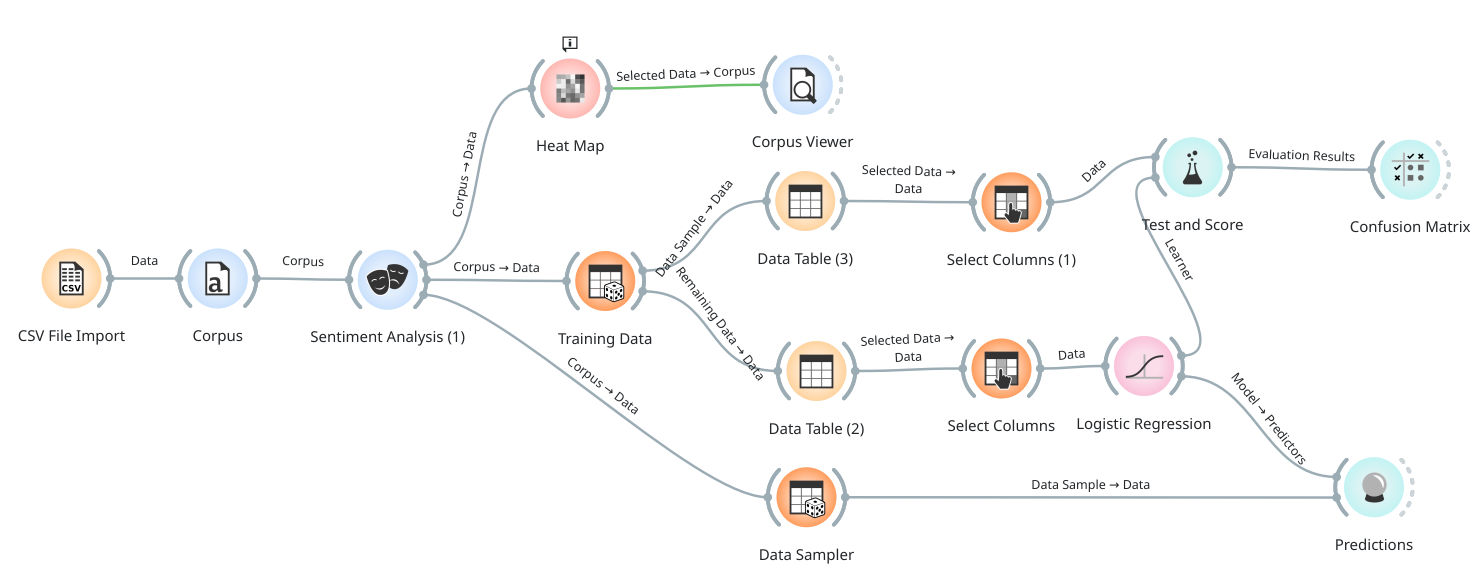
\includegraphics[width=\linewidth]{../../figures/sentiment_pipeline.png}
		\caption{Pipeline for sentiment analysis using Amazon review data from UCI}
	\end{figure}
\end{frame}

% Frame 2: Steps
\begin{frame}{Workflow Steps}
	\begin{enumerate}
		\item Import CSV/Text dataset.
		\item Convert table to Corpus for text processing.
		\item Compute sentiment scores (positive, negative, neutral, compound).
		\item Visualize with Heat Map and clustering.
		\item Split data into training/testing sets.
		\item Select sentiment scores as features, labels as targets.
		\item Train Logistic Regression model.
		\item Evaluate performance (Accuracy, Precision, Recall, F1, AUC).
		\item Display Confusion Matrix.
		\item Output predictions for new/test data.
	\end{enumerate}
\end{frame}

\begin{frame}{Sentiment Score Heatmap}
	\vspace{20pt}
	\begin{figure}
		\centering
		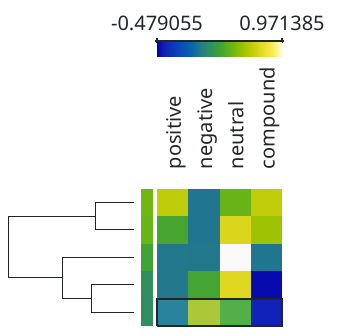
\includegraphics[width=0.4\linewidth]{../../figures/sentiment_heatmap.png}
		\caption{Heatmap of sentiment scores for \texttt{amazon\_cells\_labelled.txt} (UCI)}
		\label{fig:sentiment-heatmap}
	\end{figure}
\end{frame}

\begin{frame}{Heatmap Interpretation}
	\vspace{20pt}
	\begin{itemize}
		\item \textbf{Positive}, \textbf{Negative}, \textbf{Neutral}: proportions of respective word types.
		\item \textbf{Compound}: combined score from $-1$ (very negative) to $+1$ (very positive).
		\item Horizontal axis: score categories; vertical axis: clustered review documents.
		\item Color scale (blue → green → yellow) shows score magnitude.
		\item Black boxes mark clusters with similar sentiment patterns.
	\end{itemize}
	This helps detect sentiment trends, group similar reviews, 
	and provide context before classification.
\end{frame}

\begin{frame}{Confusion Matrix Analysis}
	\vspace{20pt}
	\begin{columns}[T,totalwidth=\textwidth]
		\column{0.5\textwidth}
		\textbf{Overview}
		\begin{itemize}
			\item Rows = \textbf{actual labels}
			\item Columns = \textbf{predicted labels}
			\item Class 0 = negative reviews
			\item Class 1 = positive reviews
		\end{itemize}
		
		\vspace{0.5em}
		\textbf{Results}
		\begin{itemize}
			\item \textbf{TN}: 45 correct negatives
			\item \textbf{FP}: 5 negatives as positives
			\item \textbf{FN}: 11 positives as negatives
			\item \textbf{TP}: 39 correct positives
		\end{itemize}
		
		\column{0.5\textwidth}
		\textbf{Interpretation}
		\begin{itemize}
			\item High accuracy; most predictions on main diagonal
			\item Only 16\% errors (5 + 11 of 100)
			\item More errors in positive reviews predicted as negative
			\item Possible conservative bias in predicting positives
		\end{itemize}
	\end{columns}
\end{frame}


\begin{frame}{Confusion Matrix Visualization}
	\vspace{20pt}
	\begin{figure}
		\centering
		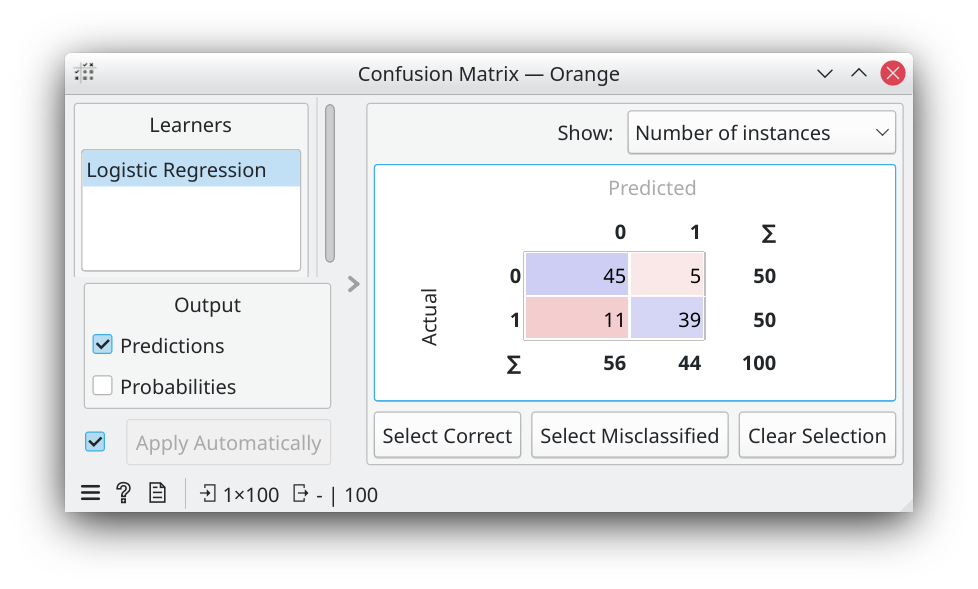
\includegraphics[width=0.6\linewidth]{../../figures/sentiment_confusion_matrix.png}
		\caption{Confusion Matrix for Logistic Regression predictions on \texttt{amazon\_cells\_labelled.txt}}
		\label{fig:sentiment-confmatrix}
	\end{figure}
\end{frame}

\begin{frame}{Model Evaluation with Test and Score}
	\vspace{20pt}
	\textbf{Validation Method:} 3-fold stratified cross-validation  
	Ensures balanced class distribution in each fold.
	
	\vspace{0.5em}
	\textbf{Metrics:}
	\begin{itemize}
		\item \textbf{AUC} = 0.931 — Excellent class separation ability.
		\item \textbf{CA} = 0.840 — 84\% accuracy on test data.
		\item \textbf{F1-score} = 0.839 — Balanced precision and recall.
		\item \textbf{Precision} = 0.845 — 84.5\% of positive predictions are correct.
		\item \textbf{Recall} = 0.840 — 84\% of actual positives detected.
		\item \textbf{MCC} = 0.685 — Strong correlation between predictions and true labels.
	\end{itemize}
	
	\vspace{0.5em}
	\textbf{Conclusion:} High AUC and stable accuracy indicate effective sentiment classification.
\end{frame}

\begin{frame}{Model Evaluation: Test and Score Results}
	\vspace{20pt}
	\begin{figure}
		\centering
		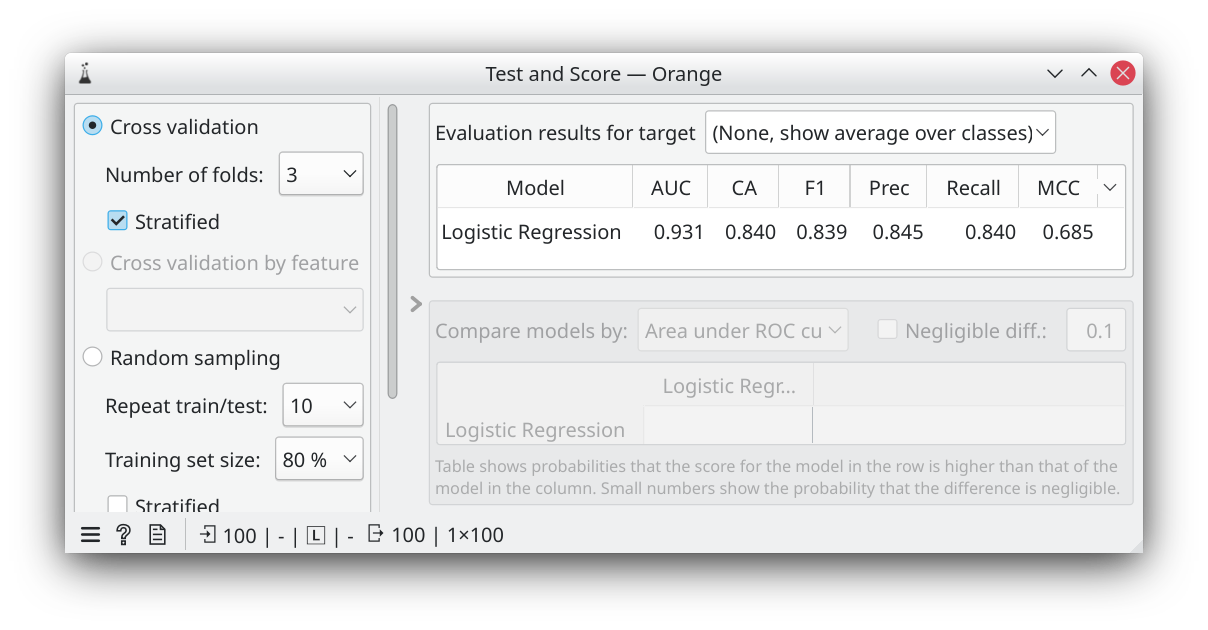
\includegraphics[width=0.75\linewidth]{../../figures/sentiment_test.png}
		\caption{Evaluation of Logistic Regression using 3-fold cross-validation on \texttt{amazon\_cells\_labelled.txt}}
		\label{fig:sentiment-testscore}
	\end{figure}
\end{frame}

\begin{frame}{Sentiment Prediction on Dataset}
	\vspace{20pt}
	\begin{itemize}
		\item Predictions widget shows model output for each review.
		\item Each row = one review from the dataset.
		\item Color represents predicted class:
		\begin{itemize}
			\item Orange = negative (0)
			\item Green = positive (1)
		\end{itemize}
		\item Useful for:
		\begin{itemize}
			\item Checking predictions on test or new data.
			\item Spotting classification patterns.
			\item Exporting results for further analysis.
		\end{itemize}
	\end{itemize}
\end{frame}

\begin{frame}{Sentiment Prediction Output}
	\vspace{20pt}
	\begin{figure}
		\centering
		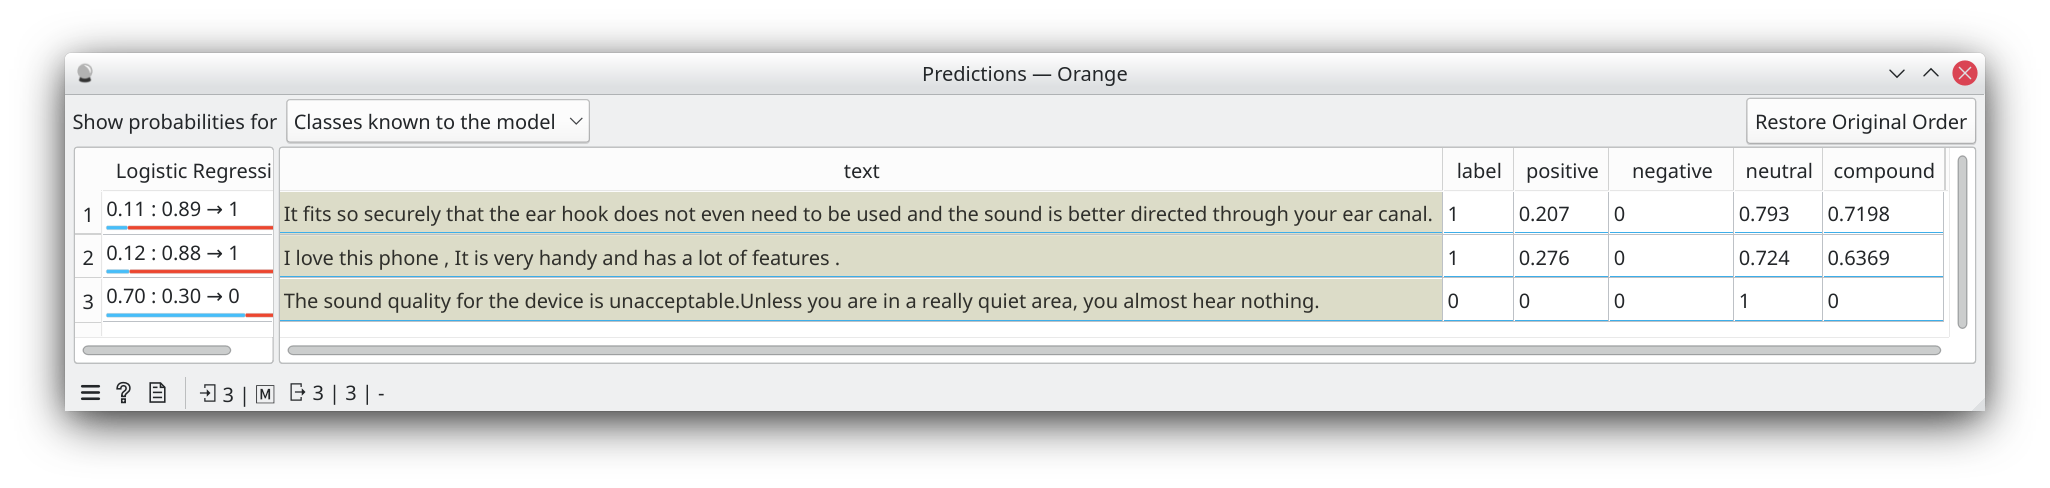
\includegraphics[width=\linewidth]{../../figures/sentiment_prediction.png}
		\caption{Predictions from Logistic Regression model on \texttt{amazon\_cells\_labelled.txt} using Orange's \textit{Predictions} widget}
		\label{fig:sentiment-predictions}
	\end{figure}
\end{frame}

\section{Interpretation and Business Strategy}
\begin{frame}{Interpretation and Business Strategy}
	\vspace{20pt}
	\textbf{Analysis Summary:}
	\begin{itemize}
		\item \textbf{Heatmap:} Identified review clusters with similar sentiment profiles (positive, negative, neutral, compound), useful for deeper cause analysis.
		\item \textbf{Model Evaluation:} AUC = 0.931, Accuracy = 0.840, F1 = 0.839, Precision = 0.845, Recall = 0.840. Indicates strong performance of Logistic Regression.
		\item \textbf{Confusion Matrix:} 84\% correct predictions; more false negatives (11) than false positives (5).
		\item \textbf{Predictions:} The 3 predictions are correct.
	\end{itemize}
\end{frame}

\begin{frame}{Business Strategy Implications}
	\vspace{20pt}
	\begin{enumerate}
		\item \textbf{Product and Service Quality Monitoring.} Analyze high negative sentiment reviews to identify recurring issues for targeted improvements.
		\item \textbf{Customer Retention Enhancement.} Use positive review patterns to pinpoint satisfaction drivers and design loyalty programs.
		\item \textbf{Customer Segmentation by Sentiment.} Leverage heatmap clustering to group customers (e.g., highly positive, mixed, highly negative) for tailored outreach.
		\item \textbf{Measuring Product Change Impact.} Compare sentiment before and after major updates to gauge effects.
		\item \textbf{Automation Integration.} Integrate the trained model into real-time monitoring to detect sentiment spikes and notify teams.
	\end{enumerate}
\end{frame}



\begin{frame}{Limitations and Future Work}
	\vspace{20pt}
	\textbf{Limitations:}
	\begin{itemize}
		\item Small, homogeneous dataset (1,000 Amazon mobile product reviews) — domain generalization untested.
		\item Lexicon-based sentiment analysis struggles with sarcasm, irony, or complex language context.
		\item Binary classification only; neutral or nuanced sentiment categories are not considered.
	\end{itemize}
	
	\vspace{0.5em}
	\textbf{Future Enhancements:}
	\begin{itemize}
		\item Use larger, more diverse datasets.
		\item Adopt deep learning models (e.g., BERT) to capture richer sentence context.
		\item Add topic modeling to identify themes behind specific sentiments.
	\end{itemize}
\end{frame}

\section{Conclusion}
\begin{frame}{Conclusion}
	\vspace{20pt}
	\begin{itemize}
		\item Text and sentiment analysis turn unstructured text into actionable insights.
		\item Key steps: data collection, preprocessing, feature extraction, and classifier choice.
		\item Approaches:
		\begin{itemize}
			\item Lexicon-based
			\item Machine learning
			\item Deep learning (e.g., BERT)
		\end{itemize}
		\item Case study: Amazon reviews in Orange.
		\item Performance: AUC = 0.931, Accuracy = 84\%.
		\item Visualizations (heatmap, confusion matrix) aid result interpretation.
		\item Business impact: quality monitoring, retention, sentiment-based segmentation.
		\item Limits: small dataset, domain-specific.
		\item Future: larger datasets, contextual models, topic modeling.
	\end{itemize}
\end{frame}


\end{document}
